%!TEX root = ../main.tex

\section{Merkle trees}
By publishing a hash of a document/data we can commit to this document, without revealing it. In the following we look at how to publish many such hashes concurrently.

\begin{example}
Given a document describing an invention, I can publish the hash of the document in a newspaper. If someone else then tries to claim my invention, I can proof that I had the document before the date in the newspaper.

This does not reveal my invention.
\end{example}

\begin{example}
In a election you can hash your vote and publish the hash of your vote. After some deadline, you can then reveal your vote to be counted.

\textbf{Problem:} An adversary can simply hash all possible values to vote for and thus discover your vote.

\textbf{Solution:} Hash vote, concatenated with random value.
\end{example}

\subsection{Committing to multiple values}
Given data $D_1$, $D_2$, $D_3$ and $D_4$. We want to commit to all four values.
We can either publish individual hashes or a single hash for all:
\begin{enumerate}[label=\alph*)]
	\item Publish $[H(D_1),H(D_2),H(D_3),H(D_4)]$.
	\item Publish $H(D_1||D_2||D_3||D_4)$.
\end{enumerate}

Variant b) requires to publish only a single hash. However to proof that $D_1$ was committed to, it is necessary to reveal also $D_2$, $D_3$, and $D_4$.

\begin{example}
We can build on scheme a) and additionally create $h_{1,2}=H(H(D_1) || H(D_2))$, 
$h_{3,4} H(H(D_3) || H(D_4))$ and $h_{1,2,3,4}= H(h_{1,2}|| h_{3,4})$.

We publish $h_{1,2,3,4}$. 

To prove that $D_3$ was included we present $D_3$, $h_4=H(D_4)$ and $h_{1,2}$.
To check the proof, recompute $h_{3,4}$ and $h_{1,2,3,4}$.
\end{example}

\begin{definition}
	A \textbf{Merkle Tree} is a (binary) tree where every note is labeled with a hash $h$.
	\begin{itemize}
		\item For internal nodes $h$ is the hash of the concatenated labels of its children ($h=H(\mathit{leftchild}.h||\mathit{rightchild}.h)$).
		\item For a leaf node, $h$ is the hash of the data stored in the node ($h=H(D_i)$).
	\end{itemize}
\end{definition}

\begin{figure}[ht]
	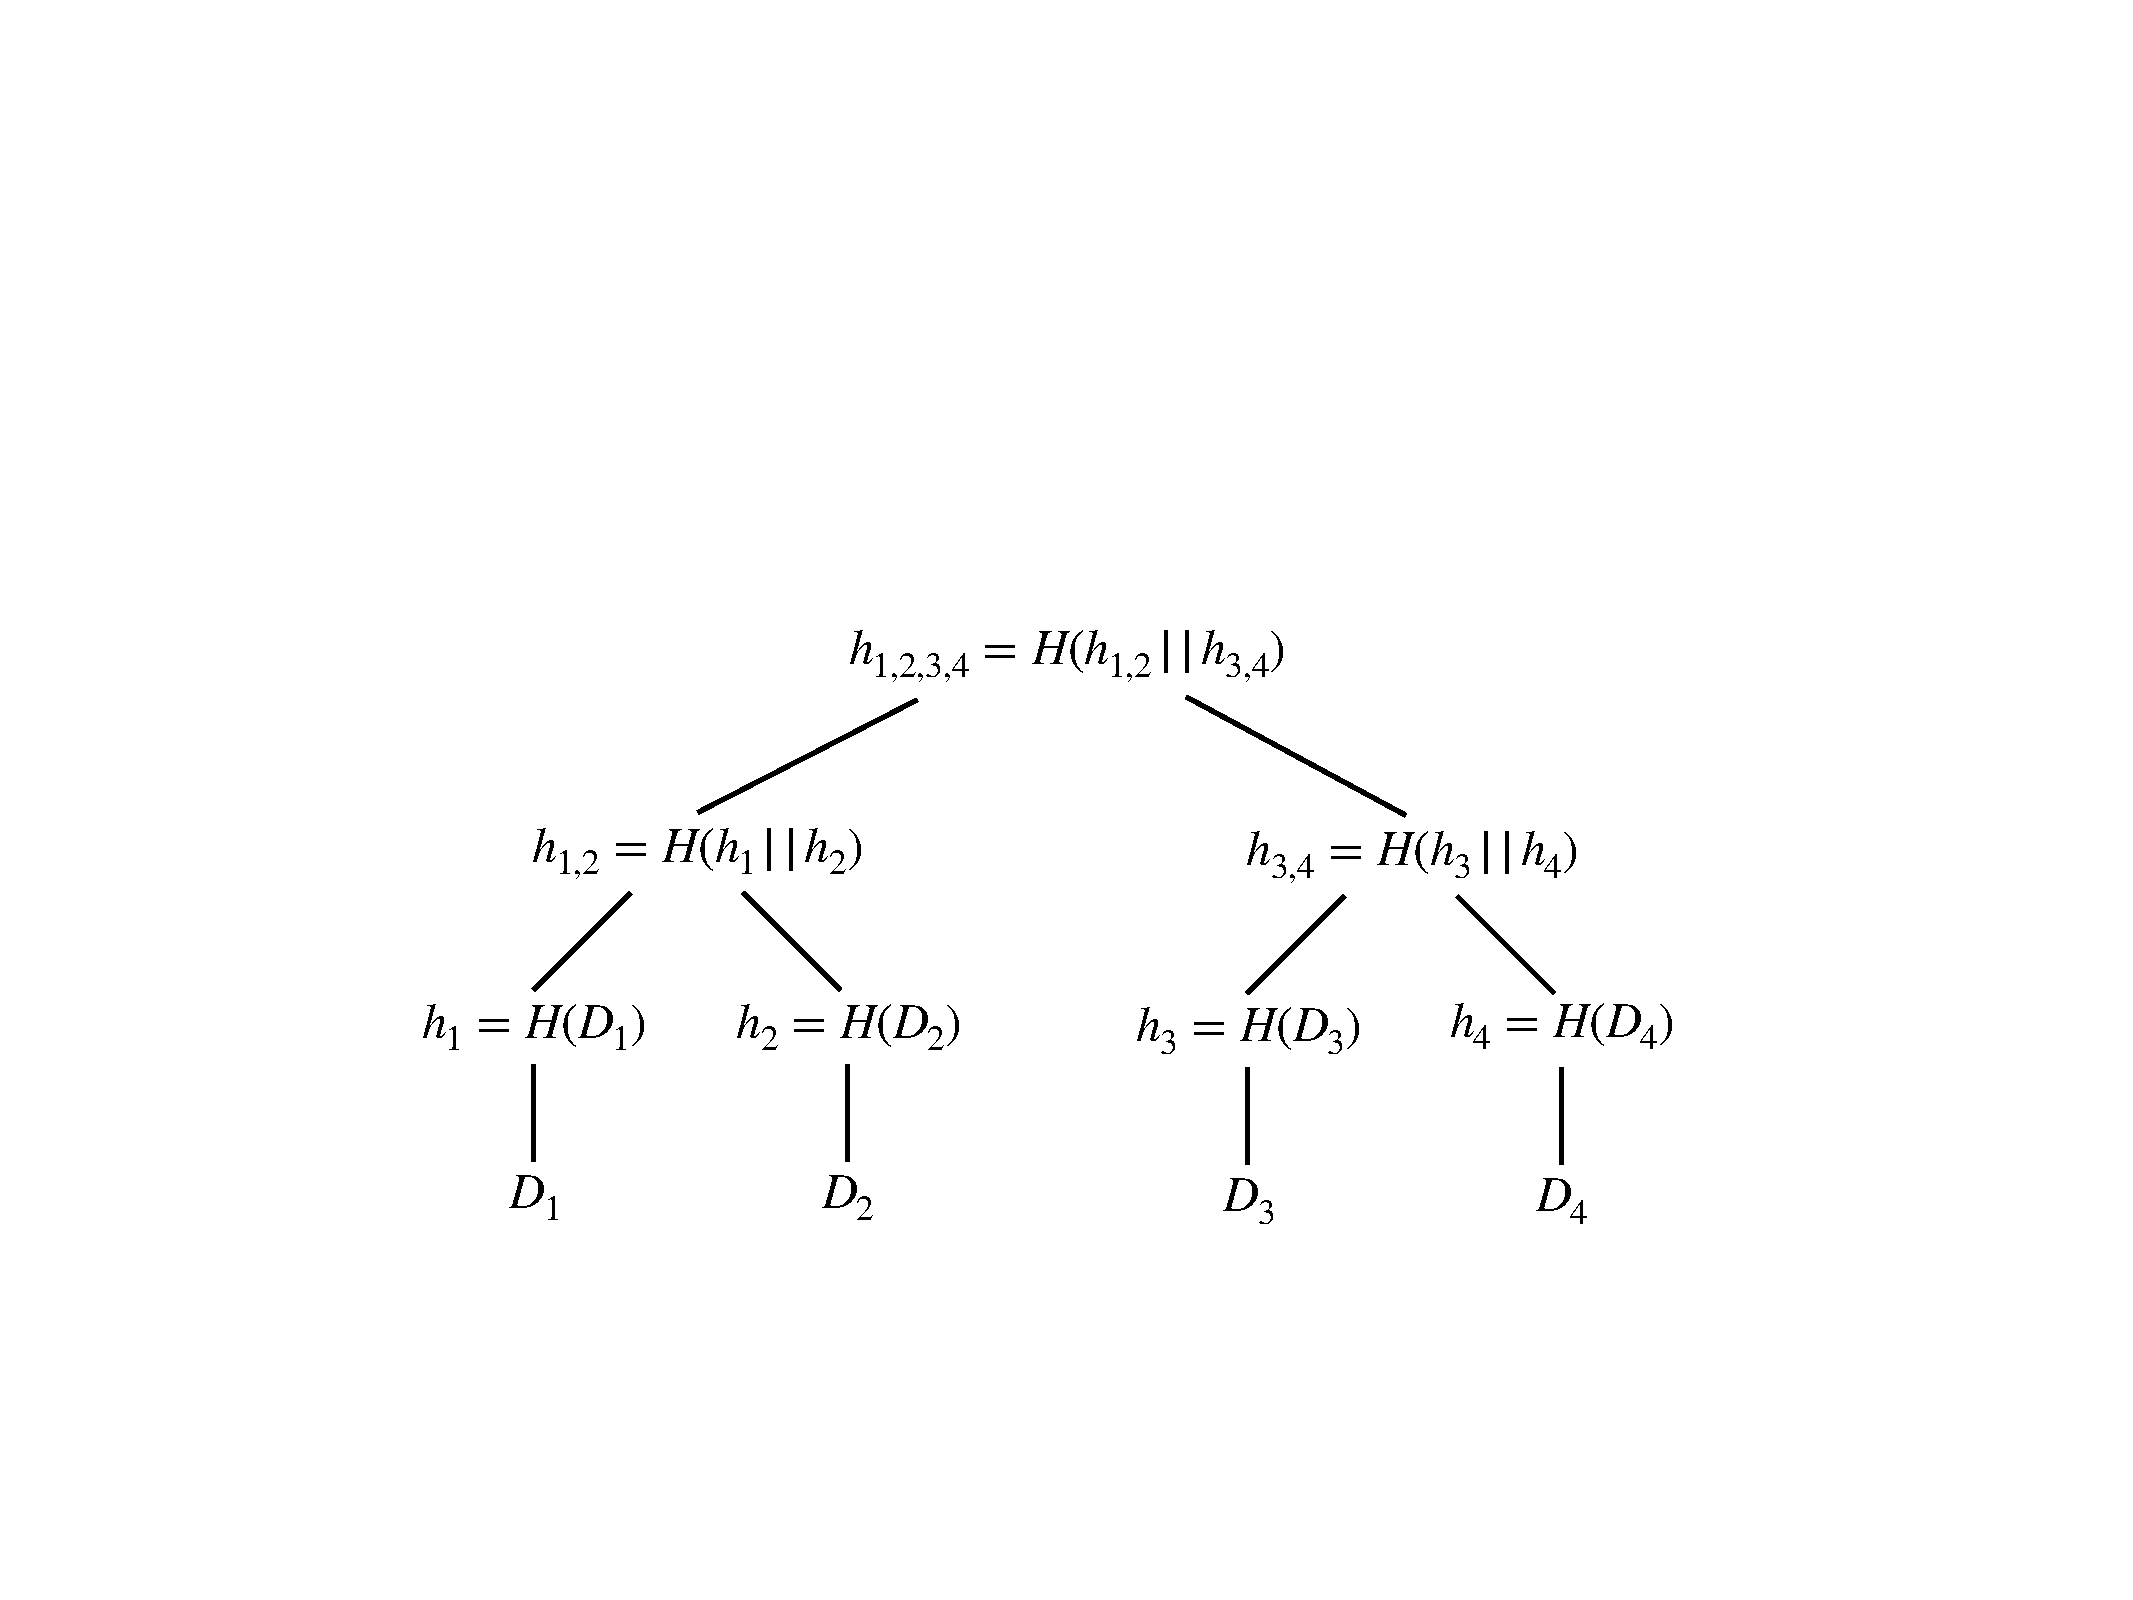
\includegraphics[width=\linewidth]{fig/merkletree}
	\caption{Merkle tree with root $h_{1,2,3,4}$}
\end{figure}

\begin{lem}
If $h_r$ is the root of a Merkle Tree with $n$ data elements, it is possible to proof that $D_i$ is one of the data elements by revealing $D_i$ and $log(n)$ node labels, i.e., hashes.
\end{lem}

\question{What is needed to recompute hashes on a path in the Merkle Tree?
\begin{itemize}
	\item Data position or
	\item Left/right information
\end{itemize}}

\begin{figure}[ht]
	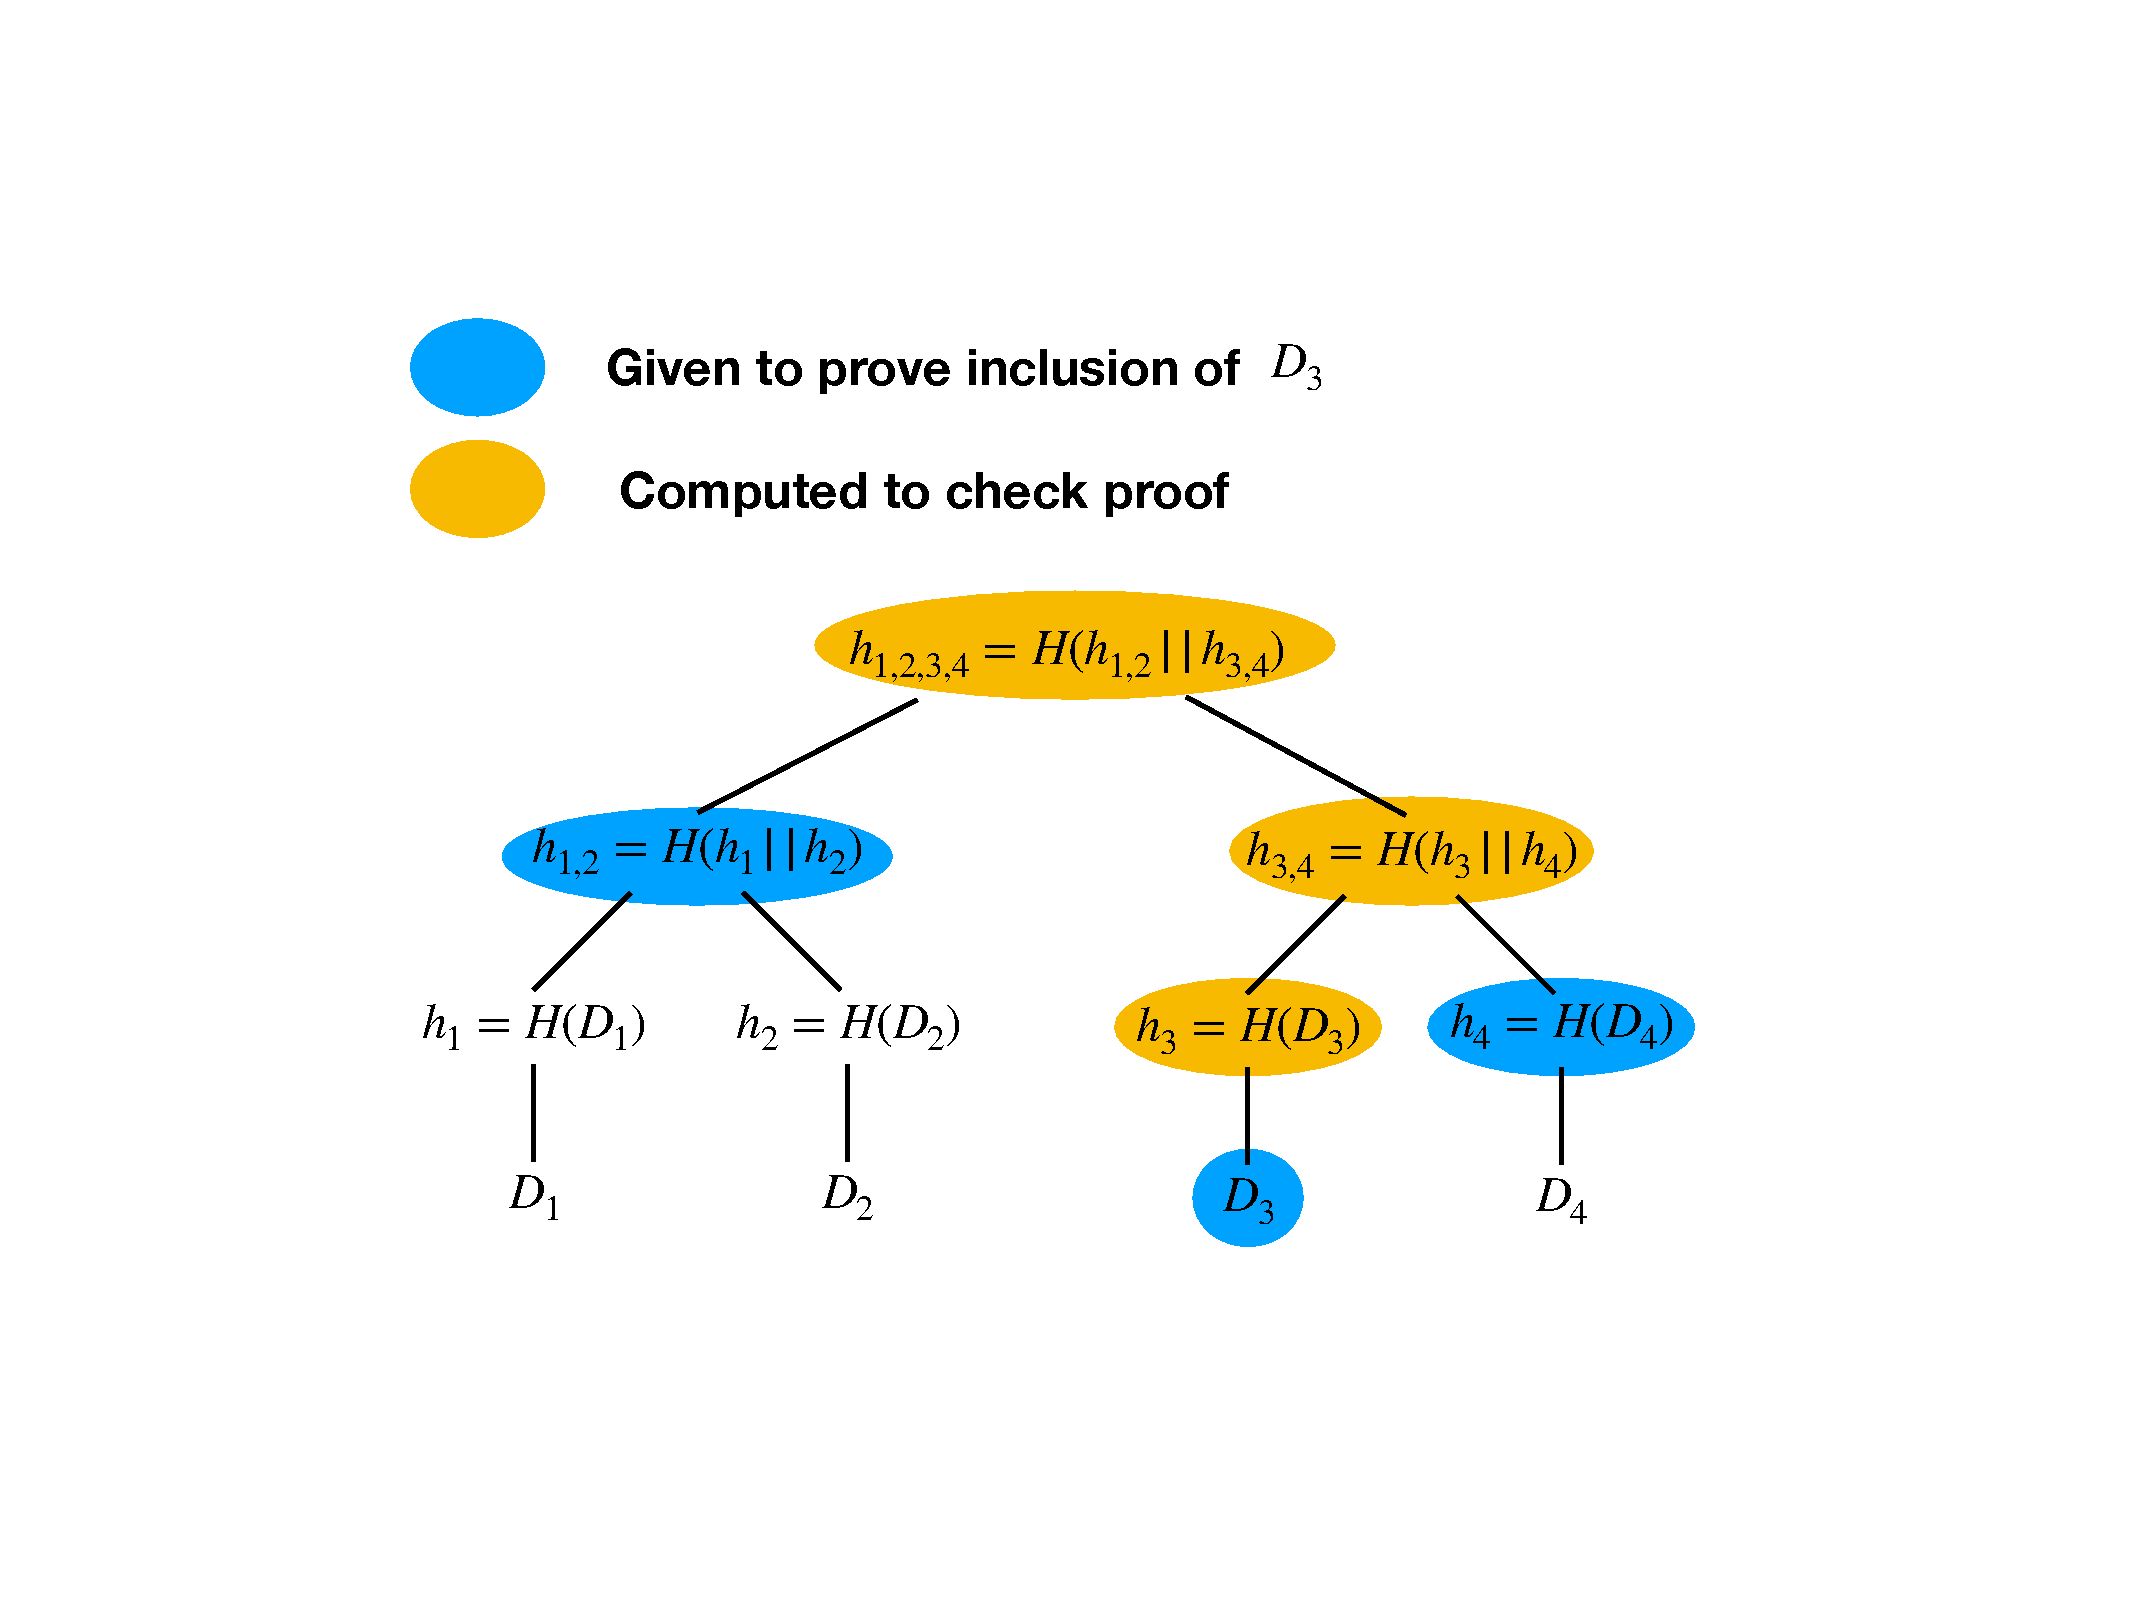
\includegraphics[width=\linewidth]{fig/merkleproof}
	\caption{Hashes necessary and computed to proof inclusion for $D_3$.}
\end{figure}

\question{How many hashes does an inclusion proof contain for a Tree with 3,8,12 or 24 data items?}

\begin{example}
	In a Merkle Tree with 16 data elements, an inclusion proof contains 4 hashes.
	
	In a Merkle Tree with 1000 data elements, an inclusion proof contains 10 hashes.
	
	In a Merkle Tree with 1 million data elements, an inclusion proof contains 20 hashes.
\end{example}

\question{Is it possible to proof that a certain document or peace of data is not included in the Merkle Tree?}

\begin{note}
It is possible to enhance other tree data-structures, e.g. binary search tree or radix tree with hashes from a Merkle tree.
\end{note}

\begin{figure}[ht]
	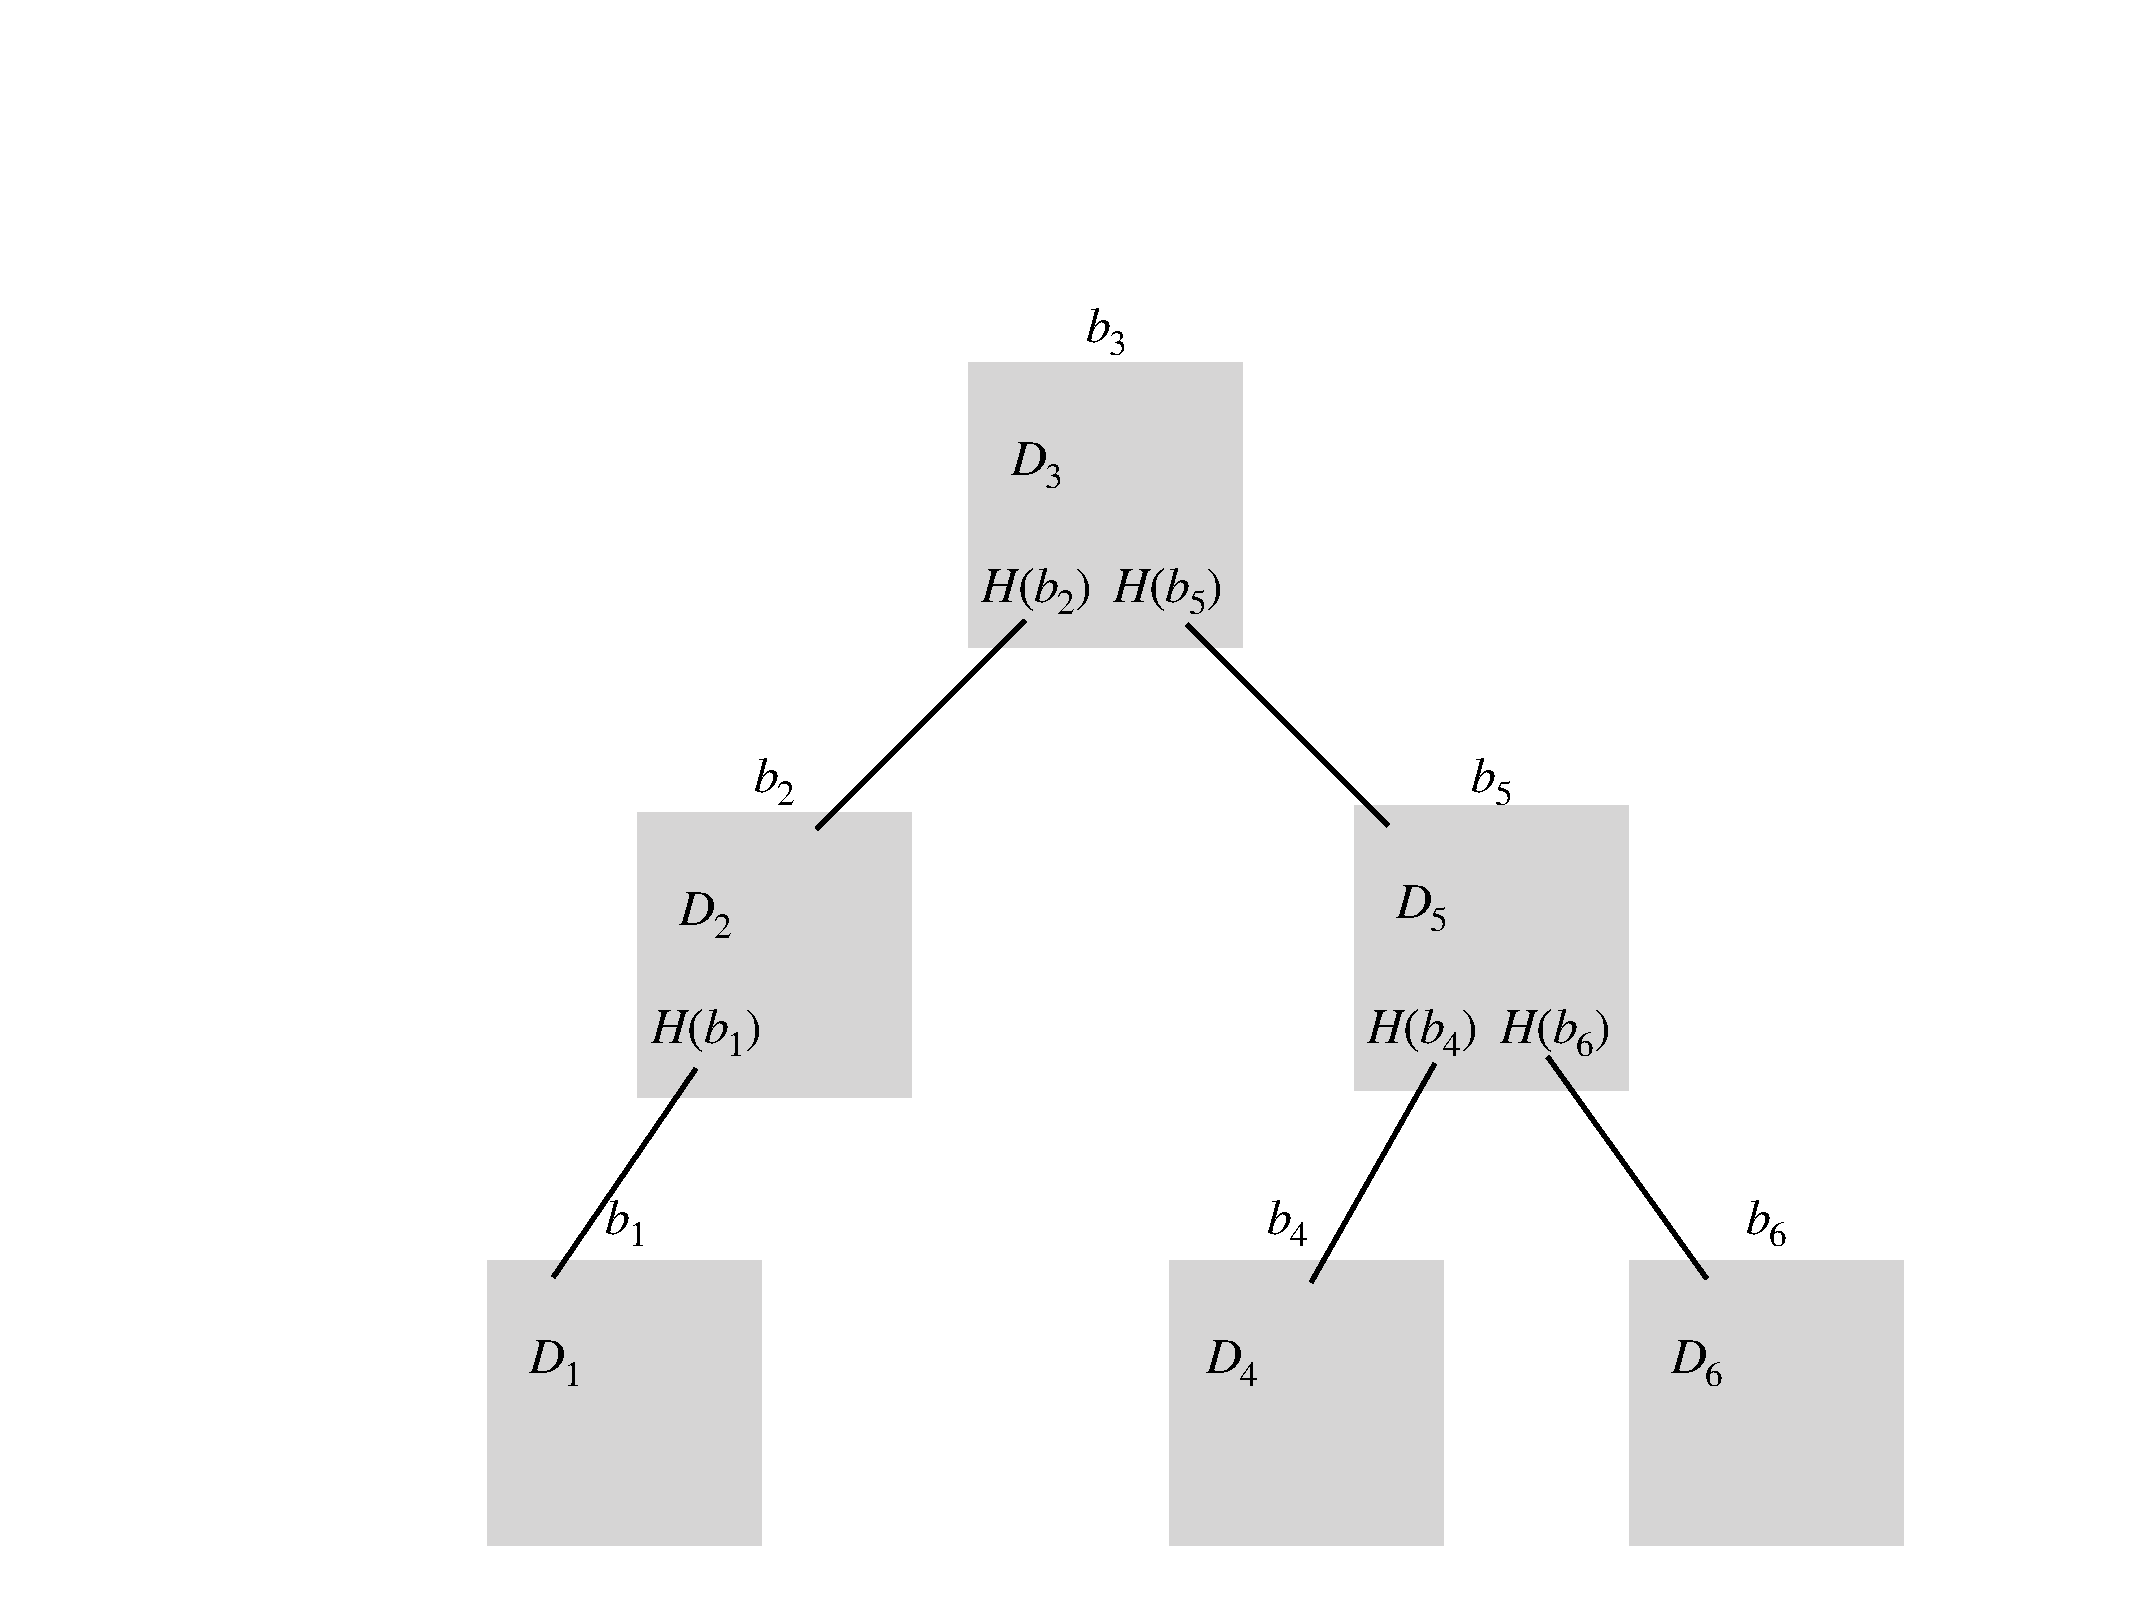
\includegraphics[width=\textwidth]{fig/binarySearchTree}
	\caption{A binary search tree enhanced with hash references.}
\end{figure}
